\documentclass[a4paper,12pt]{article}
\usepackage[utf8]{inputenc}
\usepackage{amsmath}
\usepackage{amsfonts}
\usepackage{amssymb}
\usepackage{graphicx}
\usepackage{braket}

\numberwithin{equation}{section}
\renewcommand\thesubsection{\alph{subsection}}
\newcommand{\bvp}[1]{\textbf{#1}'}
\newcommand{\bv}[1]{\textbf{#1}}

%opening
\title{Quantum I HW6}
\author{Vince Baker}

\begin{document}

\maketitle

\section{Problem 1}
The Hamiltonian of this two-level system is:
\begin{gather}
 \begin{bmatrix}
  \frac{\epsilon}{2} & \gamma\\
  \gamma    & -\frac{\epsilon}{2}
 \end{bmatrix}
\end{gather}
The energy eigenvalues are $\pm\sqrt{(\frac{\epsilon}{2})^2+\gamma^2}$.
We can write the eigenvectors in terms of an angle $\theta$, where $\tan \theta = \frac{\gamma}{\epsilon/2}$.
Then the Hamiltonian is $E\bigl ( \begin{smallmatrix}
				      \cos \theta & \sin \theta \\
				      \sin \theta & -\cos \theta
                                  \end{smallmatrix}
\bigr )$. \\
The eigenvectors are:
\begin{gather}
 \hat{e}_1= \begin{bmatrix}\cos(\frac{\theta}{2})\\ \sin(\frac{\theta}{2}) \end{bmatrix}\\
 \hat{e}_2= \begin{bmatrix}-\sin(\frac{\theta}{2})\\ \cos(\frac{\theta}{2}) \end{bmatrix}\\
\end{gather}

The state $\ket{\uparrow}$ in the eigenvector basis is:
\begin{gather}
 \ket{\uparrow}=\ket{1,0}=\ket{\cos(\frac{\theta}{2}) \hat{e}_1 -\sin(\frac{\theta}{2}) \hat{e}_2}\\
\end{gather}
The eigenfunctions evolve independently with an exponential phase factor. 
With the system starting in the $\ket{\uparrow}$ state, and $\gamma=\epsilon$, the time evolution of P10 and P01 is:

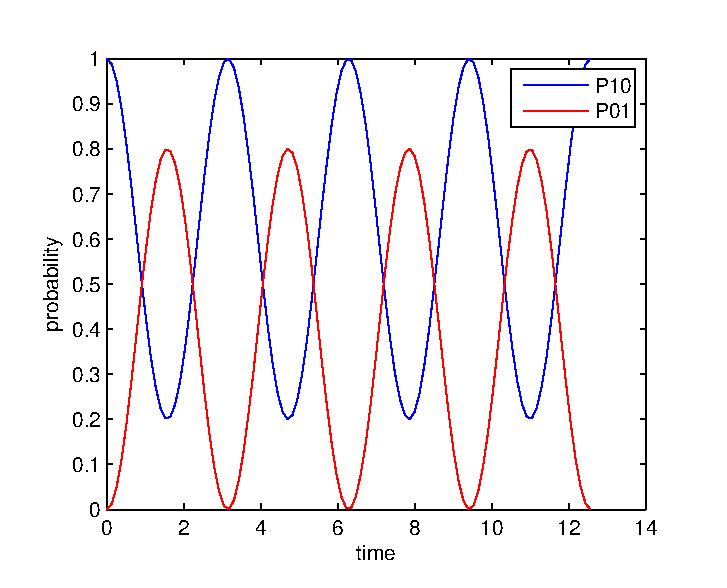
\includegraphics{p1}
\\
\section{Problem 2}
(See p2.m for work): We invert the unitary operator to find the mixture of mass eigenstates corresponding to the flavor eigenstate $\ket{1,0}$.
The Hamiltonian for the mass eigenstates is simply $\bigl( \begin{smallmatrix}c^2 & 0 \\ 0 & c^2 \end{smallmatrix} \bigr )$ and is already diagonal.
We can then evolve the mass eigenstates in time, and use the original mixing matrix to find the corresponding flavor states. 
With the given mixing angle the probability of finding the neutrino in each of the two flavors is:

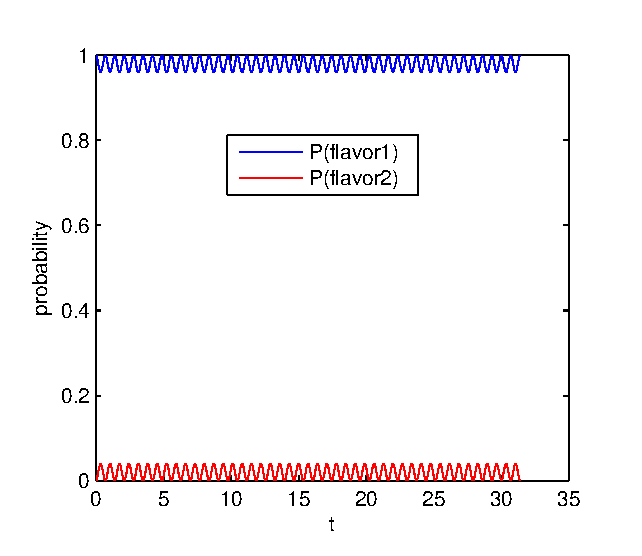
\includegraphics{p2}

\section{Problem 3}
The Hamiltonian of a time-dependent two-level system is:
\begin{gather}
 \begin{bmatrix}
  \frac{\epsilon}{2} & \gamma \cos \omega t\\
  \gamma \cos \omega t   & -\frac{\epsilon}{2}
 \end{bmatrix}
\end{gather}
The wavefunctions will have the form $\Psi = \bigl( \begin{smallmatrix}a-ib \\ c-id \end{smallmatrix} \bigr)$.
We plug this into the Schrodinger time-dependent equation and obtain (see seprate sheet) the following system of differential equations:
\begin{align}
 \frac{da}{dt}=(\frac{\epsilon}{2 \hbar})b+\frac{\gamma}{\hbar}d\\
 \frac{db}{dt}=-(\frac{\epsilon}{2 \hbar})a-\frac{\gamma}{\hbar}\cos{\omega t}\ d\\
 \frac{dc}{dt}=\frac{\gamma}{\hbar}\cos{\omega t}\ b -(\frac{\epsilon}{2 \hbar})d\\
 \frac{dd}{dt}=-\frac{\gamma}{\hbar}\cos{\omega t}\ a +(\frac{\epsilon}{2 \hbar})c\\
\end{align}
We can now integrate these equations numerically. 
With the initial state $\ket{0,1}$ the initial values are $a=0,b=0,c=1,d=0$.
With $\epsilon=\gamma=\omega=1$, the probability evolution is:\\
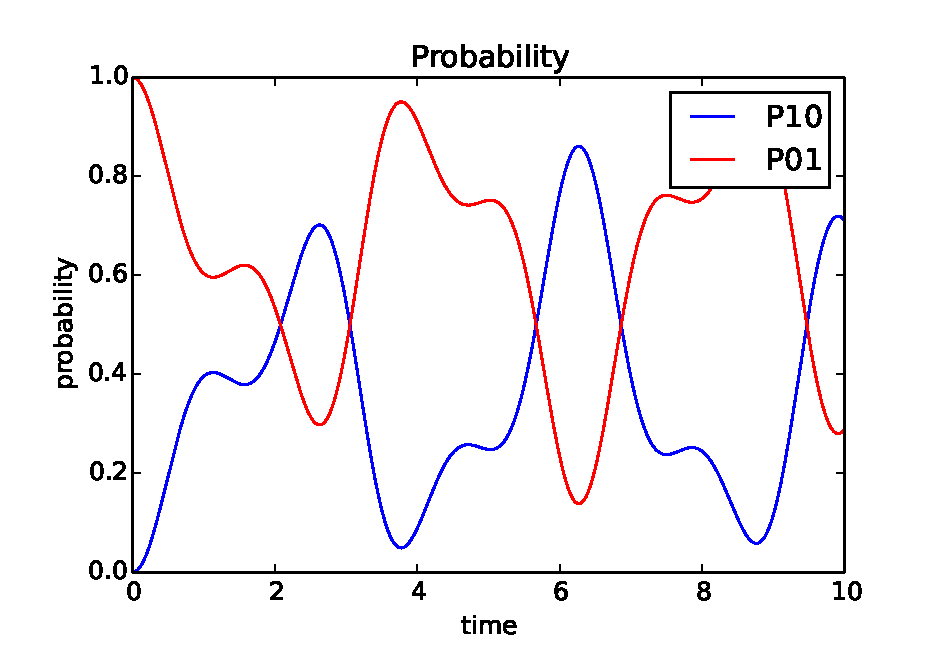
\includegraphics{p3_e1y1w1}
\\
Changing $\gamma=2$ we see:\\
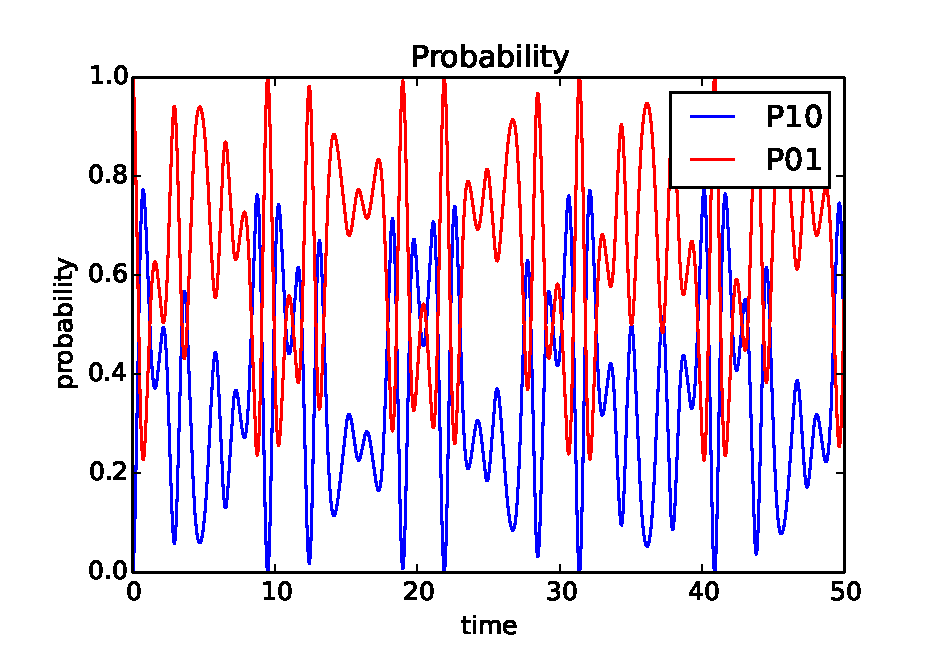
\includegraphics{p3_e1y2w1}

\section{Problem 4}
(See p4.m for work): We invert the unitary operator to find the mixture of mass eigenstates corresponding to the flavor eigenstate $\ket{1,0,0}$.
The Hamiltonian for the mass eigenstates is simply $\bigl( \begin{smallmatrix}c^2 & 0 & 0\\ 0 & c^2 & 0 \\ 0 & 0 & c^2\end{smallmatrix} \bigr )$ and is already diagonal.
We can then evolve the mass eigenstates in time, and use the original mixing matrix to find the corresponding flavor states. 
With the given mixing angle the probability of finding the neutrino in each of the two flavors is:

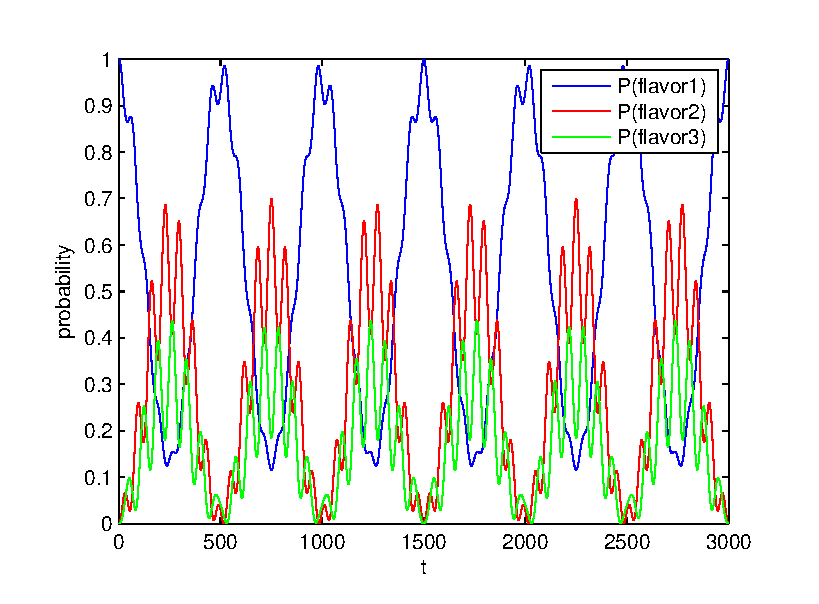
\includegraphics{p4}
\end{document}
